% ======================================== Début Préambule Latex ========================================
% Copyright (c) 2022 Mathis Gauthey
% This source code is licensed under the MIT License found in the
% LICENSE file in the root directory of this source tree.

% ========== Classe du document ==========
\documentclass[a4paper,12pt,fleqn]{report}    % A4, police taille 11, report pour avoir les chapitres, fleqn pour avoir les équations alignées à gauche

% ========== Langue française pour le document ==========
\usepackage{latexsym}       % Police latex de base

\usepackage[french]{babel}  % Dictionnaire français (indentation, caractères spéciaux, tirets...)
\usepackage[utf8]{inputenc} % Encodage d'entrée pour les caractères accentués
\usepackage[T1]{fontenc}    % Affichage correct des caractères accentués notamment

% ========== Géométrie du document ==========
% Gestion des différentes marges du document pour coller avec le séparateur d'en-tête
\usepackage[left=2cm , right=2cm, bottom=2cm, top=2cm, headheight=2cm, headsep=0.5cm,heightrounded=true]{geometry}
% \raggedbottom % This makes the last line of each page be at exactly the same place on the sheet of paper
% \flushbottom  % All pages will not necessarily have exactly the same height, but ‘almost the same height’
\setlength{\parskip}{1em}   % Définition de l'espace entre les paragraphes
\setlength{\parindent}{2em} % Définition de la longueur du "tab" = indentation
\usepackage{setspace}
\setstretch{1}
\usepackage{fancyhdr}       % Permet en-tête et pied de page
\pagestyle{fancyplain}      % Pour avoir le même style sur les pages fancy et sur celles plains comme la toc
\renewcommand\plainheadrulewidth{.4pt}  % Le trait noir sous les logos sur les pages plain
\fancyhead[L]{
\includegraphics[scale=0.05]{logo_iresne.png}}    % Logo gauche
\fancyhead[R]{
\includegraphics[scale=0.05]{polytech.jpg}} % Logo droit
% Redéfinir le style "empty" utilisé par le documentclass "report" pour le titre, résumé et chapitres
\fancypagestyle{empty}
{
    \fancyhf{}
    \fancyhead[L]{
\includegraphics[scale=0.05]{logo_iresne.png}}    % Logo gauche
    \fancyhead[R]{
\includegraphics[scale=0.05]{polytech.jpg}} % Logo droit
}

% ========== Liens dans le document, méta-datas et références ==========
\usepackage{xpatch}     % Permet de patcher certaines fonctionnalités de base comme la toc
\usepackage{float}      % Placement des flottants
\usepackage{hyperref}   % Liens dans le documents
\usepackage{caption}    % Légendes dans les environnements "figure" et "float"
\usepackage[list=true]{subcaption} % Légendes pour les "sous-figures" et "sous-float"
                                   % et affichage des "sous-..." dans la liste des figures
%\def\thechapter{\Alph{chapter}}    % Définition des chapitres avec une lettre
\setcounter{tocdepth}{3}           % Profondeur de numérotation de la toc  (chap > sec > subsec > subsubsec)
\setcounter{secnumdepth}{3}        % Profondeur de numérotation des titres (chap > sec > subsec > subsubsec)
\usepackage{chngcntr}              % Permet de changer les numérotations d'objets
\usepackage[titles]{tocloft}       % Gestion très précise des différentes listes

\hypersetup % Attribution des méta-datas pdf pour reconnaissance automatique Zotero entre autres
{
pdftitle={Titre},
pdfsubject={Sujet},
pdfauthor={Auteur},
	pdfkeywords={keyword1} {keyword2} {keyword3}
}

% ========== Graphique, police, maths ==========
\usepackage[table,xcdraw]{xcolor}       % Package permettant d'utiliser de la couleur
% \usepackage{color}                      % Rajouter de la couleur au texte
\usepackage{bm}                         % Mettre en gras des maths avec la commande \bm
\usepackage{ragged2e}                   % Meilleure gestion de l'alignement des textes entre autres
\usepackage{tcolorbox}                  % Boite colorées pour texte, images ou équations
\usepackage{textcomp}                   % Symboles et polices
\usepackage{gensymb}                    % Symbole pour le degré entre autre
\usepackage{amsmath,amsfonts,amssymb}   % Écrire des maths
\usepackage{cancel}                     % Barrer des maths
\usepackage{mathtools}                  % Gestion des matrices et de maths complexes
\usepackage{morewrites}                 % Résoud un problème entre les listes équation et codes


\usepackage{lmodern}
\usepackage[Lenny]{fncychap}

\ChNameUpperCase
\ChNumVar{\fontsize{40}{42}\usefont{OT1}{ptm}{m}{n}\selectfont}
\ChTitleVar{\Huge \bfseries}

\usepackage{pifont}
\usepackage{enumitem}       % Gestion des énumérations

% Gestion des espaces avant et après les listes plus agréable à la vue
% \setlist[itemize]{noitemsep, topsep=5pt, before={\vspace*{-\baselineskip}}}
% Si désactivé (commenté), penser à ajouter un \smallskip, \medskip ou \bigskip après un itemize.

\definecolor{bulletcolor}{RGB}{128,128,128}


\usepackage{siunitx}                                    % Pour des unités bien écrites
\newcommand{\nomunit}[1]{%
\renewcommand{\nomentryend}{\hspace*{\fill}#1}}         % Commande pour la nomenclature (unités à droite)
\sisetup{inter-unit-product =\ensuremath{{}\cdot{}}}    % Séparation par un point des unités
\DeclareSIUnit\bar{bar}                                 % Besoin de déclarer les bar car pas pris en charge

\usepackage{contour}
\usepackage[normalem]{ulem}

\renewcommand{\ULdepth}{1.8pt}
\contourlength{0.8pt}

\newcommand{\myuline}[1]{%
	\uline{\phantom{#1}}%
	\llap{\contour{white}{#1}}%
}



% ========== Glossaire ==========
%\usepackage[acronym,toc]{glossaries}    % Gestion d'un glossaire et d'une liste d'acronymes,
                                        % et ajout dans la toc de la position de ces derniers
%% Pas besoin de points à la fin du document

\newglossaryentry{mot_complexe}{
    name={mot complexe},
    description={Un mot complexe nécessite généralement une explication}}

\newacronym{lfala}{LFALA}{Les Français Aiment Les Acronymes}                        % Récupère les informations du fichier glossary.tex
%\makeglossaries                         % Génère le glossaire avec les informations récupérées

% ========== Nomenclature ==========
\usepackage[intoc]{nomencl}         % Gestion d'une nomenclature avec position dans la toc
\makenomenclature                   % Génère la nomenclature
\usepackage{etoolbox}               % Permet de créer des groupes de nomenclature

% Création de groupes de nomenclature : ATTENTION -> Uniquement des caractères uniques en identifiant
\renewcommand\nomgroup[1]{%
  \item[\bfseries
  \ifstrequal{#1}{A}{Groupe 1}{%
  \ifstrequal{#1}{B}{Groupe 2}{%
  \ifstrequal{#1}{C}{Groupe 3}{%
  }}}%
]} % Attention aux accolades lors de la création de groupes

\AtBeginDocument{   % Nomenclature à générer
\nomenclature[A]{$c_{air}$}{Célérité du son dans l'air à \SI{15}{\celsius} \nomunit{\SI{340.29}{\meter\per\second}}}
\nomenclature[B]{$T_N$}{Période propre de l'élément considéré}
\nomenclature[B]{\(E\)}{{Module d'Young}}
\nomenclature[C]{$\dot{\epsilon}$}{Vitesse de déformation \nomunit{\si{\per\second}}}
}

% ========== Gestion des figures ==========
\usepackage{graphicx}               % Plus d'arguments pour la fonction \includegraphics
\graphicspath{{Images/}}            % Path des images

%\counterwithin{figure}{section}     % Numérotation des figures à partir des sections
\setcounter{lofdepth}{2}            % Afficher jusqu'aux sous-figures dans la liste des figures
\cftsetindents{figure}{0em}{3.5em}  % Réglage de l'espace entre le numéro et le nom de la figure dans la liste
\setlength\cftbeforefigskip{5pt}    % Réglage de l'espacement entre les figures dans la liste
\AtBeginDocument{\renewcommand{\listfigurename}{Liste des figures}} % Renommer la liste des figures
% Ajout de la position de la liste des figures dans la toc
\xpretocmd{\listoffigures}{\addcontentsline{toc}{chapter}{\listfigurename}}{}{}

% ========== Gestion des tableaux ==========
\usepackage{array,multirow,makecell}                        % Packages utiles pour les tableaux
\setcellgapes{1pt}                                          % Paramètres sympa d'après Xm1Math
\makegapedcells                                             % Paramètres sympa d'après Xm1Math
\newcolumntype{R}[1]{>{\raggedleft\arraybackslash }b{#1}}   % Paramètres sympa d'après Xm1Math
\newcolumntype{L}[1]{>{\raggedright\arraybackslash }b{#1}}  % Paramètres sympa d'après Xm1Math
\newcolumntype{C}[1]{>{\centering\arraybackslash }b{#1}}    % Paramètres sympa d'après Xm1Math

%\counterwithin{table}{section}      % Numérotation des tableaux à partir des sections
\setcounter{lotdepth}{2}            % Afficher jusqu'aux sous-tableaux dans la liste des tableaux
\cftsetindents{table}{0em}{3.5em}   % Réglage de l'espace entre le numéro et le nom du tableau dans la liste
\setlength\cftbeforetabskip{5pt}    % Réglage de l'espacement entre les figures dans la liste
% Ajout de la position de la liste des tableaux dans la toc
\xpretocmd{\listoftables}{\addcontentsline{toc}{chapter}{\listtablename}}{}{}

% ========== Gestion des équations ==========
\newcommand{\listequationsname}{Liste des équations}    % Renommer la liste des équations
\newlistof{myequations}{equ}{\listequationsname}
\newcommand{\myequations}[1]{%
   \addcontentsline{equ}{myequations}{\protect\numberline{\theequation}#1}
}
\counterwithin{equation}{chapter}           % Numérotation des équations à partir des sections
\cftsetindents{myequations}{0em}{3.5em}     % Réglage de l'espace entre le numéro et le nom de l'équation dans la liste

% Création de la commande \noteworhty pour les équations importantes qui méritent d'être listées
\newcommand{\noteworthy}[2]{
\begin{align} \label{#2} \ensuremath{\boxed{#1}} \end{align}
\myequations{#2}
\begingroup
\centering \small \textit{#2}

\endgroup}

\makeatletter   % Espacement des équations plus important entre les chapitres
\xpretocmd{\@chapter}{\addtocontents{equ}{\protect\addvspace{10\p@}}}{}{}{}%
\makeatother





% ========== Index ==========
\usepackage{imakeidx}   % Package pour créer l'index
\makeindex              % Génération de l'index
% Ajout de la position de l'index dans la toc
\xpretocmd{\printindex}{\addcontentsline{toc}{chapter}{\indexname}}{}{}

% ========== Bibliographie ==========
% Importer un fichier biblatex, sans dépassement des marges, trié par ordre d'apparition
\usepackage[
backend=biber,
style=numeric,
sorting=none
]{biblatex}
\usepackage{csquotes}           % Gestion des caractères " " lors des citations
\addbibresource{biblio.bib}    % Importer le fichier de bibliographie
%\nocite{*}                      % Importer les éléments non cités quand même dans la bibliographie

% ========== Gestion des annexes ==========
\usepackage[toc,page,title,titletoc,header]{appendix}   % Packages indexes importants
\usepackage{pdfpages}                                   % Intégration de pdf dans le document
\renewcommand{\appendixtocname}{Table des annexes}      % Nom de la table des annexes dans la toc
\renewcommand{\appendixpagename}{Annexes}               % Nom du titre de la page des annexes
\usepackage{titletoc}	% Permet de générer une petite table des annexes

% ========== Utilitaires ==========
\usepackage[all,defaultlines=3]{nowidow}    % Macro pour la gestion des lignes seules en bout de page
\usepackage{blindtext}                      % Génération de texte aléatoire pour les exemples
% A utiliser avec https://ctan.mirror.garr.it/mirrors/ctan/macros/latex/contrib/mwe/mwe.pdf pour les images

% Paquets et commande perso clement plumecocq
\usepackage{bm}
\newcommand{\M}{\mathbb}					
\newcommand{\Mb}{\mathbf}									
\newcommand{\Mc}{\mathcal}
\newcommand{\grad}[1]{\nabla #1}
\renewcommand{\div}[1]{\nabla \cdot \left(#1\right)}
\newcommand{\Lapl}[1]{\Delta #1}
\newcommand{\boundary}[1]{\partial \domain{#1}}
\newcommand{\doubleoverline}[1]{\bar{\bar{#1}}} 			% notation matrice
\newcommand{\co}[1]{\text{cos}\left(#1\right)}
\newcommand{\sinus}[1]{\text{sin}\left(#1\right)}




% ======================================== Fin Préambule Latex ========================================

% ======================================== Début TUTOs ========================================

% ========== Intégrer une image ==========
%\begin{figure}[htbp]
%\centering
%\includegraphics[width=\textwidth]{example-image-a.png}
%\caption{Image A}
%\label{fig:example-image-a} % Bon réflexe de garder le même nom de fichier et de label
%\end{figure}

% ========== Insérer de multiples images ==========
% \begin{figure}[H]
%     \begin{subfigure}[t]{0.475\textwidth}
%         \includegraphics[width=1\textwidth]{example-image-b}
%         \caption{Image B}
%         \label{subfig:example-image-b}
%     \end{subfigure}%
%     ATTENTION, le % est très important ici pour éviter les problèmes de vide
%     \hfill    % Remplissage entre les images
%     \begin{subfigure}[t]{0.475\textwidth}
%         \includegraphics[width=1\textwidth]{example_image_c}
%         \caption{Image C}
%         \label{subfig:example-image-c}
%     \end{subfigure}
%     \caption{Exemple d'utilisation des sous-figures}
%     \label{fig:test_subfigure}
% \end{figure}

% ========== Placement des images ==========
% h Place the float here, i.e., approximately at the same point it occurs in the source text (however, not exactly at the spot)
% t Position at the top of the page.
% b Position at the bottom of the page.
% p Put on a special page for floats only.
% ! Override internal parameters LATEX uses for determining "good" float positions.
% H Places the float at precisely the location in the LATEX code. Requires the float package (\usepackage{float}). This is somewhat equivalent to h!, though some errors may arise if you have too many consecutive floats with [H].

% ========== Intégrer un tableau ==========
% https://www.tablesgenerator.com/

% ========== Intégrer une équation ==========
% https://editor.codecogs.com/
% \noteworthy{equation}{légende} pour l'avoir dans la liste des équations

% ========== Intégrer du code ==========
% \begin{listing}[htbp]
% \begin{minted}{c}
% #include <stdio.h>
% int main() {
%   printf("Hello, World!"); /*printf() outputs the quoted string*/
%   return 0;
% }
% \end{minted}
% \caption{Hello World in C}
% \label{listing:2}
% \end{listing}

% \mint{python}|print("hello")| % Équivalent de \minted mais plus court

% \mintinline{python}|print("hello")|   % Quand t'as qu'une ligne de code

% Remarque : Le séparateur aurait pu être { } ou d'autres ponctuations

% \inputminted[firstline=2, lastline=12]{octave}{BitXorMatrix.m}

% ========== Début de doc classique ==========
% \title{Titre}
% \author{Auteur}
% \date{\today}
% \maketitle
% \begin{abstract}
%     Blablabla
% \end{abstract}

% ======================================== Fin TUTOs ========================================
%---AUTRES PAQUETS---

%----------

\begin{document}

% ======================================== Début Page de Garde ========================================

\hypersetup{pageanchor=false}
\begin{titlepage}
    \begin{center}
        \vspace*{1cm}

        \Huge
        \textbf{Validation d'un code CFD couplant hydrodynamique et transfert de masse}

        \vspace{0.5cm}
        \LARGE
        Commisariat à l'énergie atomique et aux énergies alternatives \\
        Laboratoire de Modélisation des Accidents Graves, LMAG\\
        \Large Cadarache 13115 Saint-Paul-lèz-Durance\\
         27/02/2023 - 11/08/2023
        \vspace{1.5cm}

        \textbf{\LARGE Clément Plumecocq}

        \vfill

        
\includegraphics[scale=0.15]{logo_iresne.png}
\includegraphics[scale=0.20]{polytech.jpg}
        \vfill
        \Large
        \noindent%\fbox{\begin{minipage}[c][0.3\textwidth]{\textwidth-7pt}%
        %\begin{center}
        POLYTECH Marseille - Mécanique Énergétique \\ \vfill
        %\par\end{center}
        %\begin{center}
        Maître de stage : Romain Le Tellier, Ingénieur-Chercheur LMAG \\
        Encadrant : Mirantsoa-Aimé Rasolofomanana, Doctorant LMAG \\
        Tuteur école : 
        %\par\end{center}
        %\end{minipage}}
    \end{center}
\end{titlepage}

% ======================================== Fin Page de Garde ========================================

% ======================================== Début Page Résumé ========================================

% French

\thispagestyle{empty}
\begin{center}
    \Large


    \vspace{0.9cm}
    \textbf{Résumé}
\end{center}

\blindtext

\begin{center}
	\Large
	\vspace{0.9cm}
	\textbf{Abstract}
\end{center}

\blindtext

% ======================================== Fin Page Résumé ========================================

% ======================================== Début TOC & Co ========================================

\newpage
\hypersetup{pageanchor=true}
\setcounter{page}{1}
\tableofcontents



\newpage
\printnomenclature

% ======================================== Fin TOC & Co ========================================

% ======================================== Début Document ========================================

\newpage
\section*{Contexte et remerciements}
\chapter{Introduction}
\chapter{Présentation des accidents graves dans les réacteurs à eau pressurisée}
\section{Fonctionnement d'un réacteur à eau pressurisée}

En France 56 réacteurs nucléaires dispersés sur 18 sites sont actuellement en service, ce parc est uniquement composé de réacteur à eau pressurisée (REP). Ces réacteurs représentent 70\% de la production électrique dans l'hexagone en 2019 d'après RTE, la France étant le deuxième plus gros producteur d'énergie nucléaire dans le monde après les États-Unis. Les puissances fournies par ces réacteurs dit de deuxième génération varient entre 900 MWe et 1450 MWe. Un réacteur de troisième génération d'une puissance de 1650 MWe (EPR - European pressurized reactor) est actuellement en construction sur le site de Flamanville, ce type de réacteur prend en compte le retour d'expérience des réacteurs actuels intégrant notamment plus d'éléments de sûreté. La construction de 6 nouveaux EPR a été annoncée et 8 autres pourraient voir le jour. \\

\begin{figure}[h!]
	\centering
	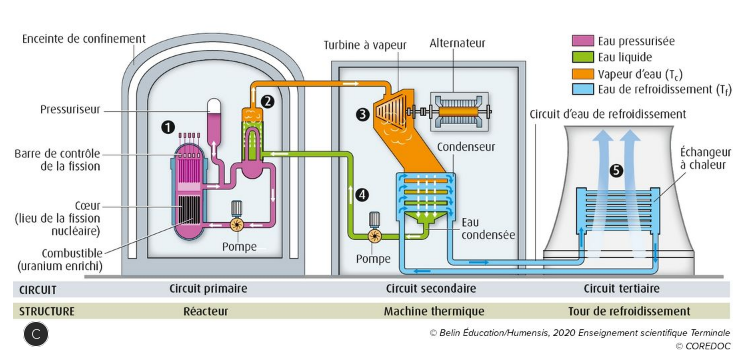
\includegraphics[width=0.8\linewidth]{figure/sch_centrale1}
	\caption[Schéma de principe d'une centrale nucléaire de type REP]{Schéma de principe d'une centrale nucléaire de type REP, (d'après manuelnumeriquemax.belin.education)}
	\label{fig:schcentrale1}
\end{figure} 
Les REP sont des réacteurs de la famille des réacteurs à eau légère, de l'eau est utilisée comme fluide caloporteur et modérateur, de plus cette eau est pressurisée à 155 bars pour éviter un changement d'état liquide-gaz dans le circuit primaire et ainsi obtenir un meilleur coefficient d'échange thermique, à l'entrée de la cuve la température de l'eau est 290\textdegree C et la température de sortie de cuve en fonctionnement nominal est de 330\textdegree C.

Le c\oe ur du réacteur est composé d'assemblages combustibles comportant chacun 264 crayons combustibles, 24 tubes pouvant contenir les crayons d'une grappe de commande ainsi qu'un tube servant à l'instrumentation. La gaine est constituée de Zircaloy qui est un alliage composé principalement de zirconium ($Zr$), les pastilles ont un diamètre de 8.2mm et sont empilées dans une gaine d'épaisseur 0.6mm et d'une longueur d'environ 4m (dépendante du palier du réacteur). Le zirconium est utilisé pour sa bonne résistance à la corrosion et sa faible absorption neutronique. Chaque c\oe ur est composé d'un ensemble d'assemblage combustible (241 pour l'EPR, embarquant au total 144.2 tonnes d'uranium enrichi) qui doivent être renouvelés périodiquement tous les 12 à 18 mois par quart ou tiers de c\oe ur.

\begin{figure}[H]
	     \begin{subfigure}[t]{0.45\textwidth}
	     	\centering
	         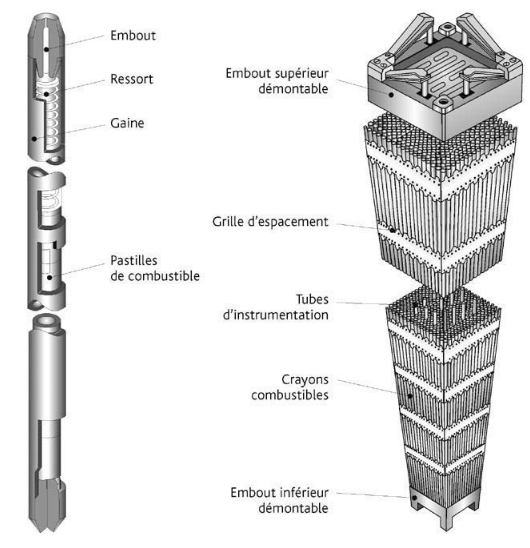
\includegraphics[width=1\textwidth]{figure/assemb.png}
	         \caption{Schéma d'un crayon combustible et d'un assemblage combustible}
	         \label{subfig:example-image-c}
	     \end{subfigure}%
     	\hfil
     	\begin{subfigure}[t]{0.45\textwidth}
     	\centering
     	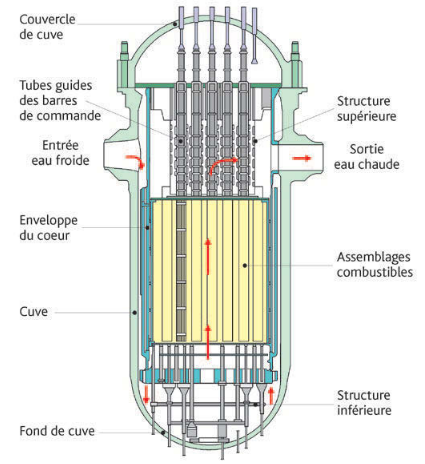
\includegraphics[width=0.99\textwidth]{figure/coeur_complet.png}
     	\caption{Schéma d'ensemble de d'une cuve d'un REP}
     	\label{subfig:example-image-c}
    	 \end{subfigure}
	     \caption{Schéma des constituants d'un c\oe ur de réacteur de type REP d'après \cite{ clement_les_2020} }
	     \label{fig:test_subfigure}
	\end{figure}
\section{Sûreté et accidents graves pour les REP}
Les questions de sûreté sont intrinsèquement liées à l'exploitation d'une centrale nucléaire tant les conséquences d'un potentiel accident peuvent être importantes. Ainsi dès le début des années 1970 le concept de défense en profondeur a été mis en place, ce concept se matérialise par la mise en place de lignes de défense successive indépendante. Pour les REP on compte 3 barrières de confinement de la radioactivité :
 \\
\begin{minipage}[c]{0.3\linewidth}
	\begin{enumerate}
		\item La gaine combustible
		\item La cuve
		\item Le bâtiment réacteur
	\end{enumerate}
\end{minipage} \hfill
\begin{minipage}[c]{0.65\linewidth}
	\centering
	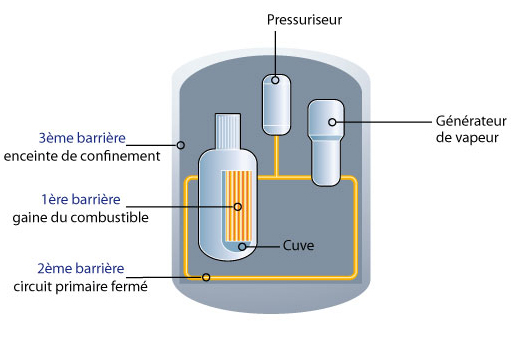
\includegraphics[width=0.7\linewidth]{figure/irsn_barriere-confinement.png}
	\captionof{figure}{Schéma des barrières de confinement (d'après irsn.fr)}
\end{minipage}
\vspace{0.5cm}


De plus les variations par rapport au régime nominal sont classés selon l'échelle INES (International Nuclear Scale Event), cette échelle permet de classifier les accidents et leurs gravités, elle comporte huit échelons allant d'un simple écart (plusieurs centaines de cas par an en France) à l'accident majeur. Les accidents correspondent aux paliers 4 à 7 et se différencient de l'incident du fait de la perte d'intégrité de la première barrière résultante de la fusion du c\oe ur, le produit de cette fusion est alors appelé corium.
\begin{figure}[h!]
	\centering
	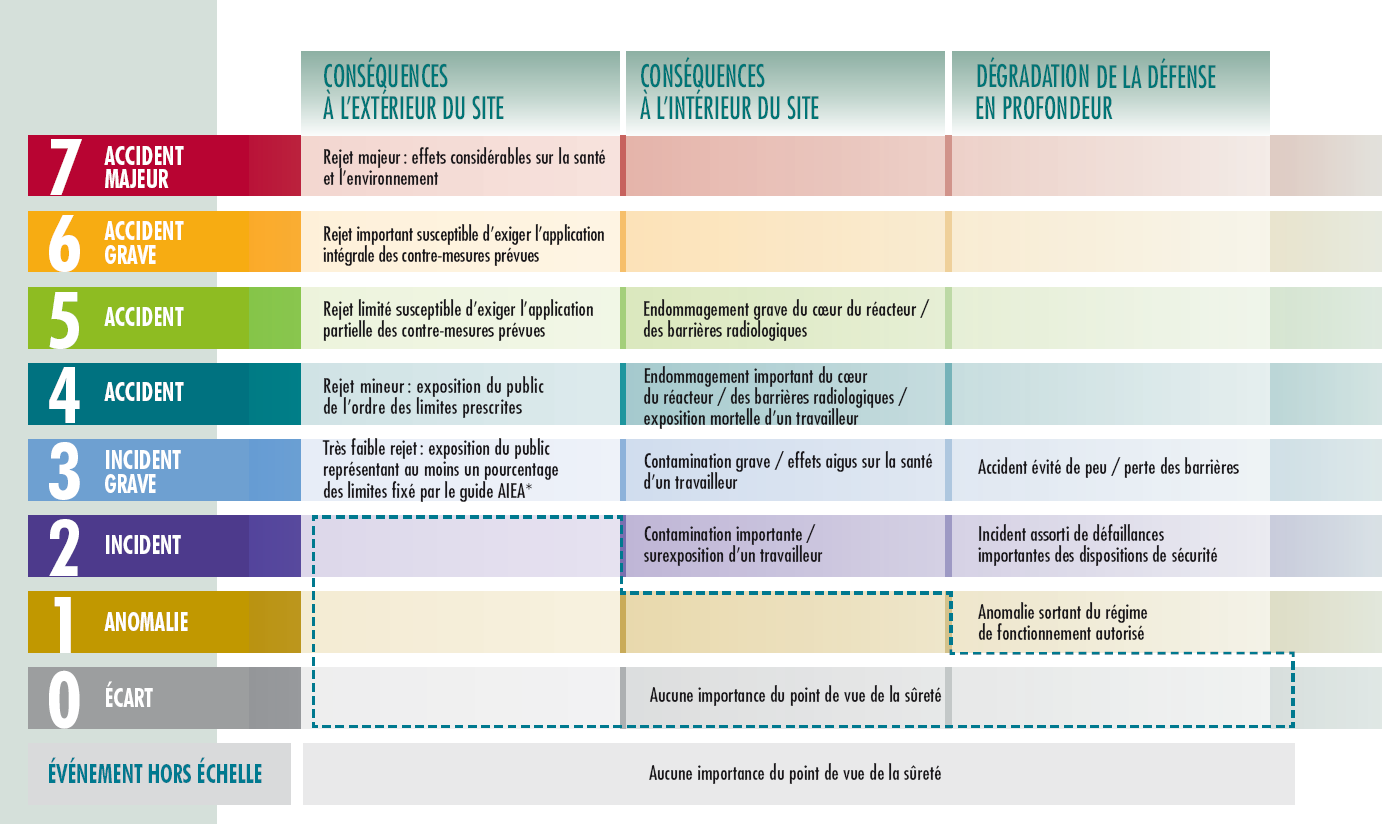
\includegraphics[width=0.7\linewidth]{figure/echelle-ines-article}
	\caption[Echelle de classification des écarts aux régimes nominal INES]{Echelle de classification des écarts aux régimes nominal INES (d'après ASN)}
	\label{fig:echelle-ines-article}
\end{figure}\\
Les accidents possibles dans les REP sont séparés en deux grandes catégories, les accidents de réactivité et les Accidents de Perte de Réfrigérant Primaire (APRP). Les accidents de réactivité sont dû à une accélération brutale de la réaction en chaîne entraînant une augmentation de puissance thermique produite. Les Accidents de Perte de Réfrigérant Primaire (APRP) résultent quant à eux d'une fuite dans le circuit primaire ou un arrêt de la circulation du fluide caloporteur. Dans la suite nous traiterons uniquement de cette seconde famille d'accident.
D'après \cite{kolev_multiphase_2015} voici le scénario de fonte du c\oe ur :
\begin{itemize}
	\item[$\bullet$] \underline{Entre 800 et 900 \textdegree C :} L'augmentation de la pression à l'intérieur de la gaine en zirconium provoque un gonflement puis une rupture de cette dernière.
	\item[$\bullet$] \underline{Entre 900 et 1300 \textdegree C :} Début de la réaction fortement exothermique d'oxydation de la gaine. A cet instant une forte proportion de la puissance thermique dégagée provient de cette réaction. La molécule d'eau est dissociée, l'oxygène est absorbé par la surface métallique et l'hydrogène est libéré. L'absorption de l'hydrogène dans les fissures du métal le fragilise davantage et accélère le processus de défaillance de la gaine. De plus l'apparition de fissure augmente la surface de réaction provoquant une accélération de la réaction.
	\item[$\bullet$] \underline{Entre 1300 et 1400 \textdegree C :} Apparition d'alliages constitués des matériaux composant la gaine (principalement Zr) et de l'acier présent dans la cuve.
	\item[$\bullet$] \underline{Entre 1400 et 1500 \textdegree C :} Fusion et rupture des structures métallique du c\oe ur. Libération des composant en phase gazeuse du combustible.
	\item[$\bullet$] \underline{Entre 1500 et 1850 \textdegree C :} Point de fusion du zirconium, dissolution du dioxyde d'uranium UO$_2$ par le zirconium en fusion, apparition de l'alliage (U,O,Zr)
	\item[$\bullet$] \underline{Entre 2000 et 2650 \textdegree C :} Fusion du ZrO$_2$, dissolution de l'UO$_2$ dans le ZrO$_2$ fondu et formation de la solution liquide UO$_2$-ZrO$_2$.
\end{itemize}
Une fois le c\oe ur fondu celui-ci se relocalise dans le fond de la cuve réacteur et il devient nécessaire d'adopter une stratégie pour refroidir ce bain.

\section{Stratégie de rétention du corium en fond de cuve (IVR)}
Une fois le c\oe ur fondu celui-ci se relocalise au fond de la cuve du réacteur. Pour limiter les conséquences d'un accident une stratégie vise à maintenir ce corium dans le fond de cette cuve, c'est la stratégie d'In-Vessel Retention (IVR). Pour cela on cherche à refroidir la cuve par l'extérieur. Cette stratégie est étudiée depuis les années 90 et mise en \oe uvre sur des réacteurs de faible puissance. \\
Le comportement du corium en fond de cuve est alors régi par deux principaux phénomènes :
La thermohydraulique du bain, avec un écoulement turbulent soumis à des rouleaux de convection (instabilité de Rayleigh-Bénard) dans la phase oxyde, d'autre part la thermochimie régit quant à elle le comportement des phases et leurs équilibres. \\
Les premières études du comportement du bain de corium ont été réalisés pour des bains stationnaires. Il a été montré qu'en régime stationnaire le bain est stratifié avec une phase oxyde et une phase métal, cependant en fonction de l'accident la couche de métal peut être lourde (i.e plus que l'oxyde et donc être en dessous) ou légère. Les différents cas sont obtenus via des différences de conditions initiales (fraction massique d'acier, degré d'oxydation du zirconium, le rapport molaire entre l'uranium et le zirconium dans la phase oxyde et la température du bain). Des études plus récentes ont montré que le transitoire reste plus contraignant et fait donc l'objet d'étude plus poussée. Lors du transitoire des phénomènes d'inversion de phase sont observés, une partie du métal de la phase légère s'alourdit sous l'effet d'un transfert de masse et des gouttes tombent, puis sous l'effet d'un même transfert de masse la phase lourde remonte. On observe alors trois couches : une couche d'oxyde, une de métal léger localiser au dessus de la couche d'oxyde et une couche de métal lourd en fond de cuve ainsi qu'une croûte située entre les phases liquides et la cuve est également présente. Finalement on se retrouve dans la situation suivante :
\begin{figure}[h!]
	\centering
	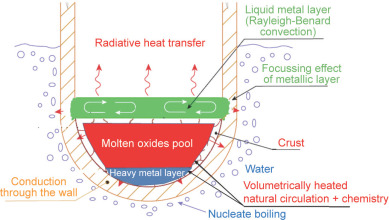
\includegraphics[width=0.6\linewidth]{figure/IVR_schema}
	\caption[Schéma du comportement du corium en fond de cuve]{Schéma du comportement du corium en fond de cuve, d'après pourlascience.fr}
	\label{fig:ivrschema}
\end{figure}\\

 

La couche de métal lourd se forme à partir d'un transfert de masse entre la phase oxyde et métal léger créant des gouttes d'acier lourd se relocalisant en fond de cuve. L'essai expérimental MASCA RCW, au cours duquel 45kg de corium ont été mis en contact avec 4kg d'acier de telle sorte que l'ensemble soit sous équilibre thermochimique dans un état de stratification comportant une phase lourde,a permis d'observer les gouttes lors de la descente, cependant la remontée de la phase lourde vers la phase légère n'a jamais été observée, l'essai ayant été arrêté au bout de 20 minutes le régime stationnaire n'a pas été atteint (voir figure \ref{fig:masca}).
 \begin{figure}[th!]
	\centering
	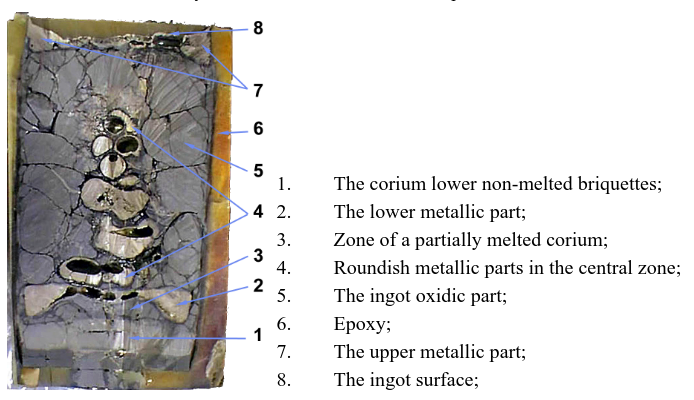
\includegraphics[width=0.7\linewidth]{figure/masca}
	\caption[Résultat MASCA-RCW 100]{Résultat MASCA-RCW 100 ,d'après \cite{}}
	\label{fig:masca}
\end{figure}


\chapter{Modélisation par une méthode champ de phase}
\section{Méthode d'interface diffuse}

Les méthodes de suivi d'interfaces peuvent se découper en deux principaux paradigmes concernant le traitement de l'interface, cette dernière peut être raide ou diffuse. Dans le second cas l'interface est modélisée comme une zone de transition d'épaisseur connue entre les deux phases ou les deux fluides cohabitent de manière à ce que les variables observées varient continuellement, facilitant ainsi le traitement numérique de l'interface, les gradients à l'interface n'étant plus infinis. Le concept d'interface diffuse date du XIX-ième siècle et est introduit par Van Der Walls sans susciter d'intérêt jusqu'au années 1950 avec la description de l'énergie libre par Ginzburg et Landau et la description thermodynamique de l'interface en utilisant cette description par Cahn et Hilliard en 1958 et 1959.
\begin{figure}[h!]
	\centering
	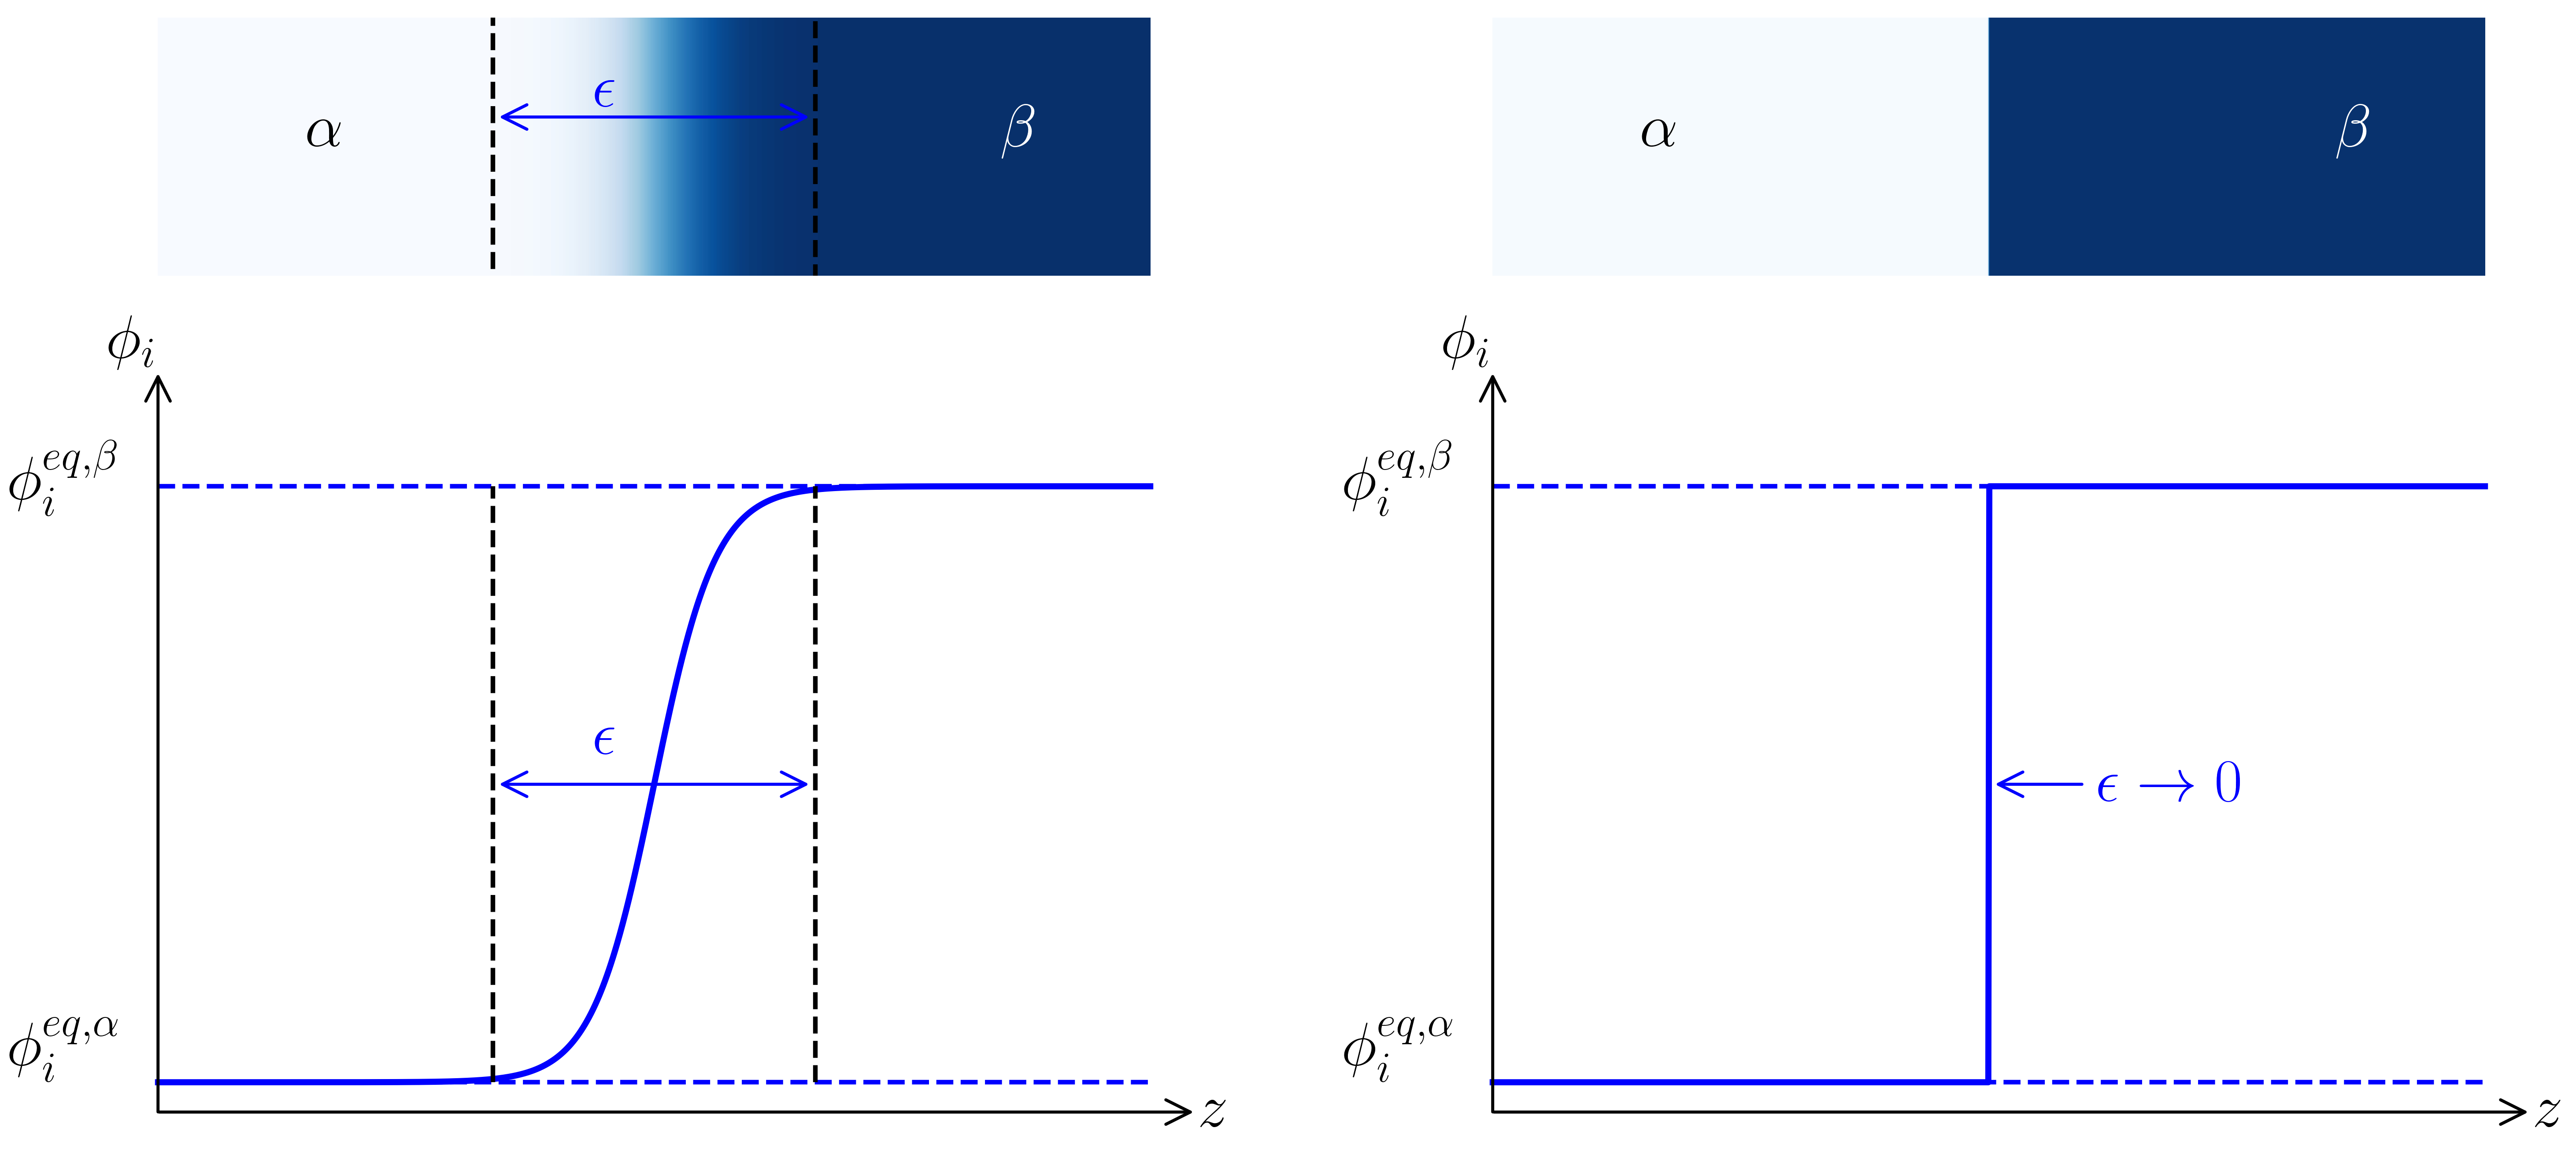
\includegraphics[width=0.3\linewidth]{figure/diffuse_interface}
	\caption[Schéma d'une interface raide et d'une interface diffuse]{Schéma d'une interface raide et d'une interface diffuse, tirée de \cite{samkhaniani_evaluation_2017}}
	\label{fig:diffuseinterface}
\end{figure} \\
L'interface est alors suivie implicitement grâce à une fonction champ de phase qui est définie à partir de grandeurs thermodynamiques. Cette fonction champ de phase prend des valeurs constantes et connues dans chaque phase. Dans la suite on notera cette variable champ de phase $\phi$. Cette méthode est utilisée dans de nombreux domaines.

\begin{figure}[h!]
	\centering
	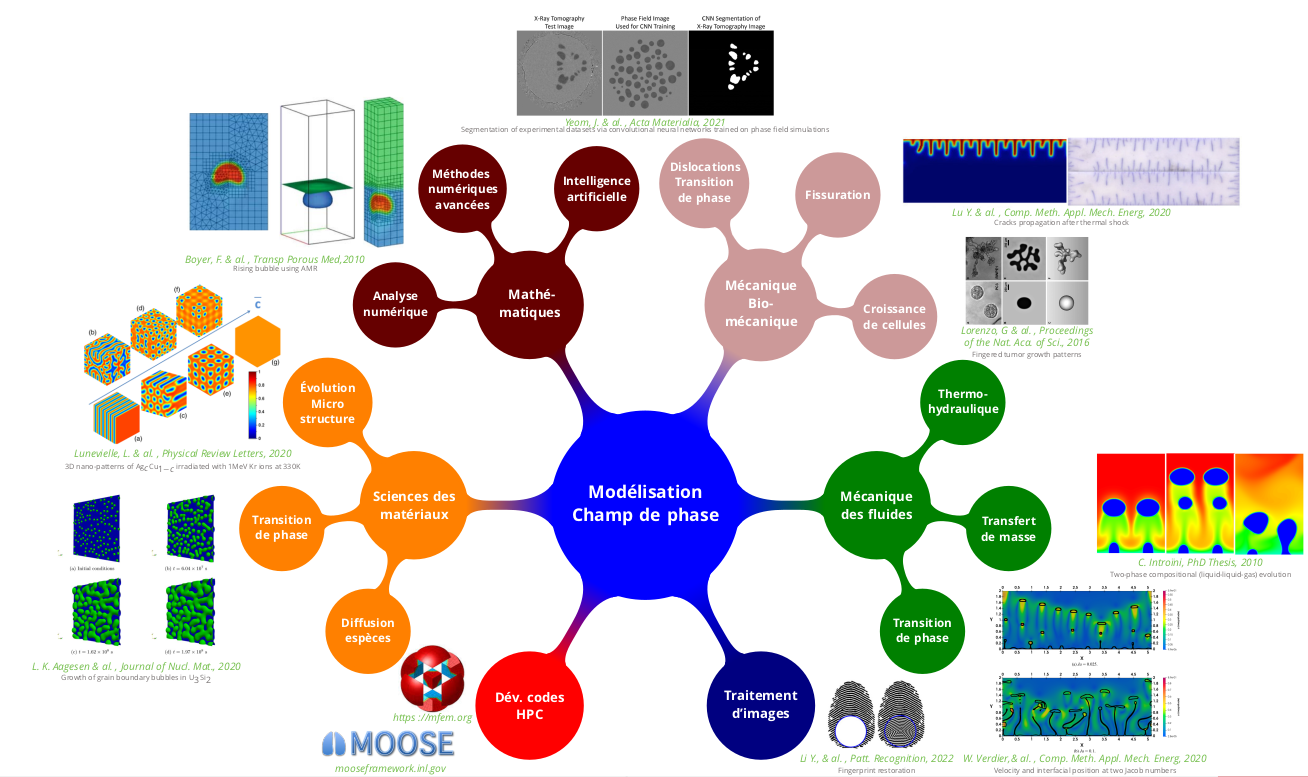
\includegraphics[width=0.9\linewidth]{figure/champ_phase}
	\caption[Domaine d'application de la méthode champ de phase]{Domaine d'application de la méthode champ de phase, tirée de \cite{introini_suivi_nodate}}
	\label{fig:champphase}
\end{figure} 
\section{Equation de Cahn-Hilliard généralisée}
Comme expliqué précédemment la méthode de champ de phase repose sur le suivi d'une variable de phase (ou paramètre d'ordre) noté $\phi_i$ pour la phase $i$ et contraint tel que : 
\begin{equation}
\sum_i \phi_i =1
\end{equation} 
Soit pour la $n$-ième phase :
\begin{equation}
\phi_n =1 - \sum_{i=1}^{n-1} \phi_i
\end{equation} 
Ainsi pour un mélange à $n$ composants, seul $n-1$ variables sont indépendantes et autant d'équations de Cahn-Hilliard sont à écrire. Dans certains cas le système peut également être décrit avec des variables non conservées telles que des indicatrices de phases ou des grandeurs liées à des réactions chimiques, les comportements de ces variables sont alors régis par une équation de réaction-diffusion dite d'Allen-Cahn, dans notre étude cette équation ne sera pas résolue car l'ensemble des paramètres d'ordre sont conservés. Dans le cadre de variables conservées les équations de Cahn-Hillard pour $n$ composants, avec $i\in \{1,..,n-1 \}$ s'écrivent sous la forme :
\begin{equation}
\cfrac{\partial \phi_i}{\partial t} + \left(\mathbf{u} \cdot \nabla\right) \phi_i=  \nabla \cdot \left(\sum_{j=1}^{n-1}{\mathcal{M}_{ij}} \nabla\left( \frac{\partial \mathbb{F}}{\partial \phi_j}\right) \right) 
\end{equation}
avec : $\mathcal{M}_{ik}$ la mobilité (paramètre cinétique),  $\phi$ le paramètre d'ordre, $\mathbf{u}$ la vitesse et $\mathbb{F}$ une fonctionnelle de Ginzburg-Landeau généralisée \cite{cardon_modelisation_2016} définit tel que : 
 \begin{equation}
\mathbb{F}[\phi_1,..,\phi_n] = \int_{\mathcal{V}}\tilde{f}_0(\bm{\phi},\mathbf{x},t)+ \sum_{i=1}^{n-1}\sum_{j=1}^{n-1}\cfrac{\kappa_{ij}}{2}\nabla \phi_i \cdot \nabla \phi_j dV
\end{equation}
Où le premier terme représente la densité d'énergie liée aux valeurs locales de composition, traduisant l'équilibre des phases ainsi que leurs existences ou coexistence. Pour deux phases $\alpha$ et $\beta$, on rappel l'équilibre thermodynamique donné par :
\begin{subequations}
	\begin{align}
		&\left.\frac{\partial \tilde{f}}{\partial \phi_i}\right|_{\phi_i^{\alpha,eq}} = \left.\frac{\partial \tilde{f}}{\partial \phi_i}\right|_{\phi_i^{\beta,eq}} = \tilde{\mu}_i^{eq} \hspace{1cm} \Leftrightarrow   \hspace{1cm} \tilde{\mu}_i^{\alpha,eq} = \tilde{\mu}_i^{\beta,eq} \\
		& 		\tilde{f}_0^{\alpha,eq} - \sum_{i=1}^{n-1}\tilde{\mu}_i^{eq}\phi_i^{\alpha,eq} = 	\tilde{f}_0^{\beta,eq} - \sum_{i=1}^{n-1}\tilde{\mu}_i^{eq}\phi_i^{\beta,eq}
	\end{align} 
\end{subequations}
Le second terme représente la contribution des interfaces, le coefficient $\kappa$, dit coefficient de gradient, tient compte du coût énergétique engendré par l'interface, par la suite ce paramètre pourra être relié à la tension de surface. \\
Finalement la dérivé variationnelle de cette fonctionnelle d'énergie libre peut être définit comme un potentiel de diffusion $\tilde{\mu}$: 
\begin{equation}\label{eq_potentiel}
	\frac{\partial \mathbb{F}}{\partial \phi_j} =\lambda \frac{\partial \tilde{f}_0}{\partial \phi_j} -\sum_{k=1}^{n-1} \kappa_{jk} \Delta \phi_k = \tilde{\mu}_j
\end{equation}
avec $\lambda$ un paramètre d'upscalling numérique ajouté pour augmenter l'épaisseur de l'interface, dans le cas où $\lambda=1$ l'interface est d'épaisseur "réelle" soit de l'ordre de l'angstr\oe m, les capacités de calcul ne permettant pas de pouvoir faire des calculs avec des maillages contenant de si petits éléments. \\
Le potentiel de diffusion peut être relier au potentiel chimique tel que :
\begin{equation}
	\tilde{\mu}_i = \frac{1}{V_m}\left(\mu_i - \mu_n\right)
\end{equation}
Avec $\tilde{\mu}_i$ (en J.m$^{-3}$) représente le potentiel de diffusion de l'élément $i$, et $V_m$ le volume molaire supposé constant dans tout le système.\\
Le potentiel chimique étant classiquement définit tel que :
\begin{equation}
	\mu_i = \left.\frac{\partial G}{\partial n_i}\right|_{P,T,n_{j\neq i }} = \left.\frac{\partial F}{\partial n_i}\right|_{V,T,n_{j\neq i }}
	  \textrm{                        où           } F = V_m f_0
\end{equation}
Avec $F$ (resp. $G$) l'énergie libre d'Helmotz (resp. Gibbs) (en J) et $n_i$ la quantité de matière de l'élément $i$ (en mol). Dans notre cas on se place dans une transformation isobare et isotherme, on privilégiera donc l'énergie de libre de Gibbs.
Dans le cas où $\doubleoverline{\kappa}$ = $\doubleoverline{0}$ on retrouve une équation d'advection-diffusion classique, dans le cas contraire on obtient une équation d'ordre 4. Une des principale difficulté dans la mise en place de méthode champ de phase repose sur le paramétrage des simulations.
\section{Couplage avec les équations de Navier-Stokes incompressible}
Dans le cadre de cette étude les équations de Cahn-Hilliard sont couplées aux équations de conservation de masse et de quantité de mouvement incompressible sous l'approximation de Boussinesq, d'après \cite{kim_phase-field_2012} le système d'équations s'écrit sous la forme :
\begin{subequations}
\begin{align}
&\nabla \cdot \mathbf{u} = 0\\
&\rho^* \left (\frac{\partial \mathbf{u}}{\partial t} + (\mathbf{u} \cdot {\nabla})\mathbf{u}\right) = -{\nabla} P +\eta \Delta \mathbf{u}+\sum_{i=1}^{n-1} \tilde{\mu}_i{\nabla} \phi_i + \rho(\bm{\phi}) \mathbf{g}
\end{align}
\end{subequations}
avec $\mathbf{u}$ la vitesse, $P$ la pression, $\mu_i$ le potentiel chimique du composant $i$, $\mathbf{g} = \{ 0,0,-g\}^T $, $\eta$ la viscosité cinématique supposée constante, $\rho^*$ la masse volumique du solvant \\
La densité est alors calculé : 
\begin{equation}
	\rho(\bm{\phi}) = \rho^*\left(1+\sum_{i=1}^{N-1}\beta_i \phi_i\right)
\end{equation}
Les paramètres $\beta$ sont à déterminer en fonction du système étudié, $\rho_0$ correspond à une masse volumique de référence. L'équation de Cahn-Hilliard étant d'ordre 4, une résolution implicite est alors préférée pour les simulations.
\section{Paysage thermodynamique analytique}
L'objectif présenté dans \cite{noauthor_numerical_nodate} est de d'obtenir une formulation analytique du terme homogène de la fonctionnelle de Ginzburg-Landau. Dans le cas binaire, cette contribution est de la forme d'un double puit d'ordre 4.
\begin{figure}[h!]
	\centering
	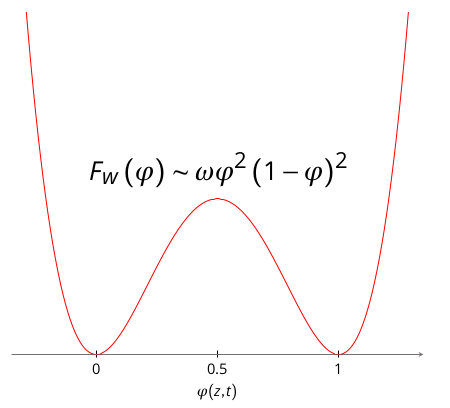
\includegraphics[width=0.4\linewidth]{figure/DP}
	\caption[Exemple d'une contribution homogène à l'énergie]{Exemple d'une contribution homogène à l'énergie, d'après \cite{introini_suivi_nodate}}
	\label{fig:dp}
\end{figure}\\
L'objectif est de généraliser ce double puit pour un système ternaire, ainsi on introduit un pseudo grand potentiel correspondant à l'énergie nécessaire pour changer de minimum d'énergie \cite{cardon_modelisation_2016}.
\begin{equation}
\Omega^{\star} =\Omega - \Omega^{eq} =  \tilde{g}^{liq} - \sum_i \tilde{\mu}_i^{eq}\phi_i - \left(  \tilde{g}^{liq,eq} -  \sum_i \tilde{\mu}_i^{eq}\phi_i^{eq} \right) 
\end{equation}
Les bases thermodynamiques étant peu développées aux points d'intérêt (Température supérieure à 2000 \textdegree C) on cherche à définir ce potentiel grâce à une formulation analytique que l'on note :
\begin{equation}\label{double_puit}
	\Omega^{\star}  = P^{dis} \times P^{cont}
\end{equation}
Où $P^{dis}, P^{cont}$ représente deux paraboloïdes correspondant à la phase dispersée et continue. Dans le cas ternaire, avec les éléments $A$ et $B$ d'intérêt, les paraboloïdes sont de la forme : 
\begin{multline}
	P^{k}=\left(\frac{\co{\theta^{k}}(\phi_{A}-\phi_{A}^{eq,k}) + \sinus{\theta^{k}}(\phi_{B}-\phi_{B}^{eq,k})}{a_{A}^{k}}\right)^{2}+\\ \left(\frac{-\sinus{\theta^{k}}(\phi_{A}-\phi_{A}^{eq,k}) + \co{\theta^{k}}(\phi_{B}-\phi_{B}^{eq,k})}{a_{B}^{k}}\right)^{2}
	\label{eq:paraboloid_general_}
\end{multline} 
Avec $k = \{disp,cont\}$ la phase (dispersée ou continue), $a_A$ (respectivement $a_B$) le demi-grand (resp petit) puits, $\theta_k$ l'angle de rotation associé au puits de la phase $k$\\
On cherche alors à tracer ce paysage.
\begin{figure}[h!]
	\centering
	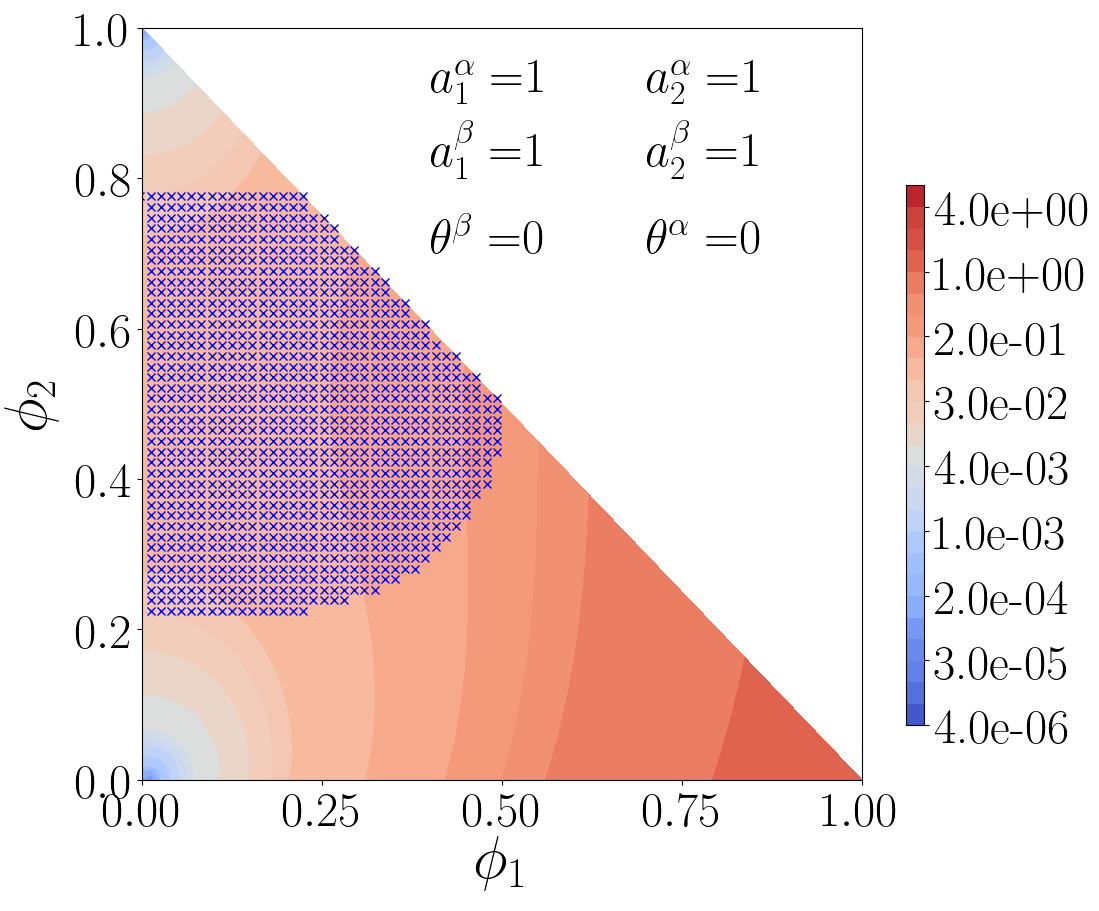
\includegraphics[width=0.7\linewidth]{figure/landscape}
	\caption{Exemple de paysage thermodynamique, en rouge la droite reliant les concentration initiales et en bleu la droite reliant les concentrations à l'équilibre, les pointillés réprésentant la zone instable présenté ci-dessous}
	\label{fig:landscape}
\end{figure}
On peut dès lors calculer le potentiel de diffusion homogène grâce à la formulation analytique (\ref{double_puit}) :
\begin{align}
	\tilde{\mu}_i & \nonumber= \frac{\partial}{\partial \phi_i}\left\lbrace 
	\Omega^{\star} + \sum_j \tilde{\mu}_j^{eq}\phi_j + \left( {g}^{liq,eq} -  \sum_j \tilde{\mu}_j^{eq}\phi_j^{eq} \right)\right\rbrace \\
	&\nonumber = \frac{\partial \Omega^{\star}}{\partial \phi_i} + \frac{\partial g^{liq,eq}}{\partial \phi_i} + \sum_j \frac{\partial \tilde{\mu}_j^{eq}\left(\phi_j - \phi_j^{eq}\right)}{\partial  \phi_i}\\
	\tilde{\mu}_i &=	P^{dis}\frac{\partial P^{cont}}{\partial \phi_i} + P^{cont}\frac{\partial P^{dis}}{\partial \phi_i} + \tilde{\mu}_i^{eq}
\end{align} 
%\begin{align*}
	%& \frac{\partial g^{liq,eq}}{\partial \phi_i} = 0 \\
		%& \sum_j \frac{\partial \tilde{\mu}_j^{eq}\left(\phi_j - %\phi_j^{eq}\right)}{\partial  \phi_i} = \tilde{\mu}_i^{eq} %+\tilde{\mu}_{j\neq i}^{eq} \frac{\partial \phi_{j\neq i}}{\partial %\phi_i} = \tilde{\mu}_i^{eq}
%\end{align*}
L'objectif est alors de déterminer les paramètres des paraboloïdes pour obtenir des résultats consistants thermodynamiquement.
\section{Éléments de stabilité de phase}
Dans le cadre de notre étude nous nous intéressons à deux phases en coexistence, une phase dite continue et l'autre dispersée. La détermination de la stabilité des phases est essentielle pour pouvoir tracer le paysage thermodynamique. La courbe binodale correspond à la condition pour laquelle deux phases peuvent coexister, c'est-à-dire que sous la courbe binodale le système peut être composé d'une seul phase, il le sera dans la zone instable et pourra l'être dans la zone métastable.
\begin{figure}[h!]
	\centering
	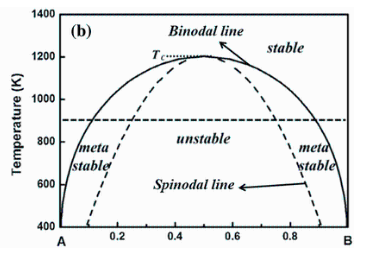
\includegraphics[width=0.5\linewidth]{figure/metastable}
	\caption[Exemple de diagramme de stabilité de phase pour un cas binaire, d'apres]{Exemple de diagramme de stabilité de phase pour un cas binaire, d'apres}
	\label{fig:metastable}
\end{figure}
Cependant le calcul de la zone instable est beaucoup plus simple que celui de la zone métastable. Pour déterminer cette zone instable on calcul la matrice Hessienne définit tel que : 
\begin{equation}
	\Mb{\doubleoverline{H}}_{g^{liq}} = \left.\frac{\partial^2 g^{liq}}{\partial \phi_i \partial \phi_j}\right|_{T,P,\phi_k\neq i,j}
	=\left.\frac{\partial^2 \Omega^{\star}}{\partial \phi_i \partial \phi_j}\right|_{T,P,\phi_k\neq i,j}
\end{equation}
L'égalité des matrices hessienne du pseudo-grand potentiel et de l'énergie libre de Gibbs est ici immédiate. D'après \cite{aursand_spinodal_2017} les zones spinodale, instable et stable sont définit tel que :
\begin{itemize}
	\item zone stable : $\displaystyle eig\left\{\Mb{\doubleoverline{H}}_{g^{liq}} \right\} > 0$, deux phases coexistent \\ 
	\item spinodale : $\displaystyle \min \left( eig \left\{\Mb{\doubleoverline{H}}_{g^{liq}}\right\} \right) > 0$, décomposition spinodale \\
	\item zone instable : $\displaystyle eig\left\{\Mb{\doubleoverline{H}}_{g^{liq}} \right\} < 0$, une phase en présence \\ 
\end{itemize}
Le calcul des valeurs propres en chaque point du paysage pouvant être coûteux on rappel que par théorème le produit des valeurs propres d'une matrice est égale au déterminant de cette matrice. Ainsi si on note $\lambda_i$ les valeurs propres de $\Mb{\doubleoverline{H}}_{g^{liq}}$ on a :
\begin{equation}
	\det{\Mb{\doubleoverline{H}}_{g^{liq}}} = \prod_i \lambda_i
\end{equation}
Pour le cas ternaire le calcul du déterminant est direct :
\begin{equation}
	\text{det}  \Mb{\doubleoverline{H}}_{g^{liq}}   =  \frac{\partial^2 g^{liq}}{\partial \phi_i^2}
	\frac{\partial^2 g^{liq}}{\partial \phi_j^2}-\left(\frac{\partial^2 g^{liq} }{\partial \phi_i \partial \phi_j} \right)^2
\end{equation}
Ainsi la zone instable correspond à la zone où le determinant de la matrice hessienne est négatif.


\section{Expérience numérique}

L'objectif est de réaliser numériquement l'expérience proposée par Abhijit Rao et al. dans \cite{rao_influence_2015}. Pour cette expérience une goutte composée d'Acetonitrile et de Chlorobenzene est placée dans de l'eau. l'acetonitrile est miscible dans l'eau contrairement au chlorobenzene qui est immiscible. Initialement la goutte est plus légère que l'eau environnante et monte puis sous l'effet du transfert de masse la densité de la goutte augmente jusqu’à une inversion du rapport de densité conduisant à la redescente de la goutte.
\subsection{Choix des conditions initiales}
Les conditions initiales choisies pour la concentration sont de la forme tangente hyperbolique.
\begin{equation}
	\phi_{i}(\mathbf{x},t=0) = \frac{\phi^{init,cont}_i + \phi^{init,disp}_i  }{2} +  \frac{\phi^{init,cont}_i - \phi^{init,disp}_i }{2}\tanh\left(\cfrac{\sqrt{(x-x_0)^2+(y-y_0)^2}-R}{\varepsilon} \right)
\end{equation}
Avec ($x_0$, $y_0$) les coordonnées du centre de la goutte, $R$ le rayon de la goutte, $\varepsilon$ l'épaisseur de l'interface (paramètre numérique) et $\phi_i^{init,cont}$ (resp. $\phi_i^{init,disp}$) la concentration initiale de l'élément $i$ dans la phase continue (resp. dispersée) .\\
Cette solution analytique provient d'un problème avec une interface plane (sans courbure), dans la littérature il n'existe pas de solution analytique pour une interface courbée, l'effet de Gibbs-Thomsom n'est donc pas pris en compte, ainsi on observe un léger mouvement de l'interface lors du premier pas de temps. \\
Pour s'assurer de la sphéricité de la goutte lors de la simulation on calcule le nombre adimensionné de Bond  représentant le ratio entre les forces de gravité et la tension de surface tel que :
\begin{equation}
	Bo = \cfrac{\Delta \rho g D^2}{\sigma}
\end{equation}
avec $\Delta\rho$ la différence de densité entre les deux phases, $D$ le diamètre de la goutte et $\sigma$ la tension de surface.\\
On considère que pour $Bo \ll 1$ la tension de surface domine et la goutte reste sphérique.
\begin{figure}[h!]
	\centering
	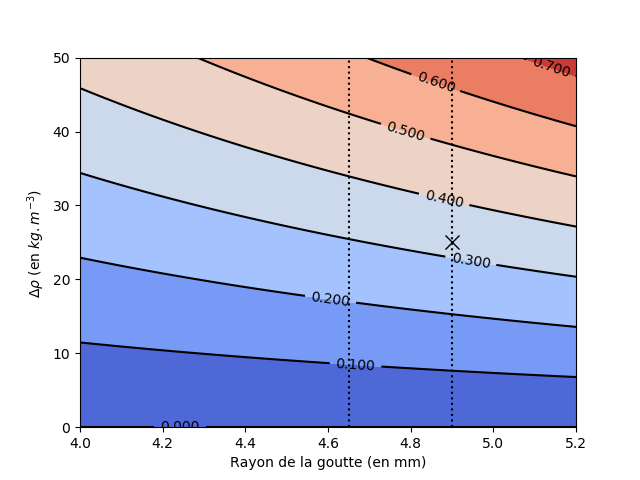
\includegraphics[width=0.7\linewidth]{figure/contour_bond}
	\caption[Valeur du nombre de Bond en fonction de la différence de densité et de la tension de surface entre les phases]{Valeur du nombre de Bond en fonction de la différence de densité entre les phases et le rayon de la goutte, le marqueur représente l'état initial}
	\label{fig:contourbond}
\end{figure}\\
Il est alors possible, dans notre cas, de discuter de la sphéricité de la goutte au vu de la valeur ici $Bo = 0.32$

% ======================================== Fin Document ========================================

% ======================================== Début Listes & Co ========================================


\newpage
\printbibliography
\begin{appendix}
\chapter{Solution analytique pour une interface plane}
La solution analytique stationnaire permet de donner des conditions initiales cohérentes, ainsi on s'intéresse au cas binaire "classique" (avec un seul paramètre d'ordre noté $\phi$), La densité d'énergie est choisit de la forme analytique d'ordre 4 en double puits :
\begin{equation}
	f(\phi) = \phi^2 (1-\phi)^2
\end{equation}
La fonctionnelle de Ginzburg-Landau est alors de la forme :
\begin{equation}
	\mathbb{F} =\int_V \lambda f(\phi) + \frac{1}{2}\kappa ||\nabla \phi||^2 dV
\end{equation}
Avec $\lambda$ un paramètre d'upscalling présenté précédemment, $\kappa$ un coefficient de gradient.
Dans l'état stationnaire, la condition d'équilibre nous donne :
\begin{equation}
	\kappa \frac{d^2\phi}{dz^2} = \lambda \frac{d f(\phi)}{d\phi}
\end{equation}
L'astuce est alors de multiplier l'équation par $\displaystyle \frac{d\phi}{dz}$ puis d'intégrer entre 0 et $L$, soit :
\begin{align}
	& \kappa \frac{d^2\phi}{dz^2}\frac{d\phi}{dz} = \lambda \frac{d f(\phi)}{d\phi}\frac{d\phi}{dz} \\
	\Rightarrow & \kappa \int_0^z \frac{d^2\phi}{dz^2}\frac{d\phi}{dz} dz= \int_0^z \frac{d f(\phi)}{dz} dz
\end{align}
Loin de l'interface, en $z=0$ on considère le système à l'équilibre soit $\frac{d\phi}{dz} = 0$ et on fixe une condition au limite de type Dirichlet homogène :
\begin{equation}
	\phi (z= 0) = 0 \Rightarrow f(0) = 0
\end{equation}
Finalement le résultat de l'intégration précédente nous donne :
\begin{equation}
		\frac{1}{2}\kappa \left(\frac{d\phi}{dz}\right) = \lambda f(\phi)
\end{equation}
En remplaçant $f(\phi)$ par sa formulation analytique : 
\begin{equation}
	\frac{d\phi}{\phi(1-\phi)} = \sqrt{\frac{2\lambda}{\kappa}} dz
	\label{solution_statio_plane}
\end{equation}
En posant $u = 2\phi - 1$ soit $du = 2d\phi$
\begin{align*}
	 \cfrac{d\phi}{\phi(1-\phi)} &= \cfrac{\cfrac{1}{2}du}{\left(\cfrac{u+1}{2}\right)\left( 1 -\cfrac{u+1}{2}\right)} \\
	 & = \frac{2du}{(1+u)(1-u)} \\
	 & = 2\frac{du}{1-u^2}
\end{align*}
Finalement l'équation \ref{solution_statio_plane} devient :
\begin{equation}
	\frac{du}{1-u^2} = \cfrac{1}{2}\sqrt{\frac{2\lambda}{\kappa}}dz
\end{equation}
On remarque que le termes de gauche correspond à la dérivée de la fonction réciproque de la tangente hyperbolique, soit :
\begin{equation}
	\text{arctanh}(u) = \cfrac{1}{2}\sqrt{\frac{2\lambda}{\kappa}} z + C
\end{equation}
Avec $C$ une constante d'intégration.
En réutilisant le changement de variable il est immédiat que :
 \begin{equation}
 \phi(z) = \frac{1}{2}\left(\tanh \left(\cfrac{1}{2}\sqrt{\frac{2\lambda}{\kappa}}z +C\right)+1\right)
 \end{equation}
La constante $C$ peut être déterminé à partir d'une valeur moyenne du paramètre d'ordre, cette résolution ne sera pas explicité ici.

\chapter{De la tension de surface au coefficients de gradient}
\section{Méthode générale}
Cette deuxième annexe présente la méthode de calcul des coefficients de gradient à partir de la tension de surface qui est une donnée physique du système. Physiquement la tension interfaciale $\sigma$ représente l'excès d'énergie libre par unité de surface associé à la présence d'une interface entre deux phases distinctes, on peut ainsi la écrire :
\begin{equation}
\sigma = \cfrac{\mathbb{F}-\mathbb{F}^{hom}}{S}
\end{equation}
Où $S$ représente la surface de l'interface, $\mathbb{F}$ l'énergie libre du système et $\mathbb{F}$ l'énergie libre homogène du système, c'est-à-dire l'énergie libre du système dénuée d'interface. 
Dans un premier temps on rappel la forme des fonctionnelles de Ginzburg-Landau associées à ses deux systèmes :
\begin{align*}
&\mathbb{F} = \int_{V}\sum_{i=1}^{n-1}\sum_{j=1}^{n-1}\frac{\kappa_{ij}}{2}\nabla \phi_i \cdot \nabla \phi_j + f(\phi_1,..,\phi_{n-1}) - \sum_{1}^{n-1}\tilde{\mu}_i^{eq}\phi_i dV \\
&\mathbb{F}^{hom} = \int_V f^{\alpha,eq}  - \sum_{1}^{n-1}\tilde{\mu}_i^{eq}\phi_i^{\alpha,eq} dV 
\end{align*}
Ainsi en combinant les deux équations précédentes : 
\begin{equation}
\sigma = \int_{V}\sum_{i=1}^{n-1}\sum_{j=1}^{n-1}\frac{\kappa_{ij}}{2}\nabla \phi_i \cdot \nabla \phi_j + f(\phi_1,..,\phi_{n-1}) - f^{\alpha,eq} - \sum_{1}^{n-1}\tilde{\mu}_i^{eq}(\phi_i-\phi_i^{\alpha,eq}) dV
\end{equation}
Dans le cas 1D suivant $z$ l'équation précédente devient : 
\begin{equation}
\sigma = \int_{0}^L\sum_{i=1}^{n-1}\sum_{j=1}^{n-1}\frac{\kappa_{ij}}{2}\frac{ d\phi_i}{dz} \frac{ d\phi_j}{dz} + f(\phi_1,..,\phi_{n-1}) - f^{\alpha,eq} - \sum_{1}^{n-1}\tilde{\mu}_i^{eq}(\phi_i-\phi_i^{\alpha,eq}) dz
\end{equation}
La condition d'équilibre s'écrit :
\begin{equation}
\sum_{j=1}^{n-1} \kappa_{i,j} \frac{d^2\phi_j}{dz^2} = \left.\frac{\partial f}{\partial \phi_i}\right|_{\phi_{j\neq i}} - \tilde{\mu}_i^{eq}
\end{equation}
Après multiplication par $\displaystyle \frac{d\phi_i}{dz}$ et intégration on trouve :
\begin{equation}
\sigma = \int_0^L \sum_{i=1}^{n-1}\sum_{j=1}^{n-1} \kappa_{i,j}\frac{d\phi_i}{dz}\frac{d\phi_j}{dz}dz
\end{equation}
On retrouve alors la relation permettant la détermination de ce coefficient dans le cas binaire en posant $n=2$
\begin{equation}
\sigma = \int_0^L\kappa^{bin}\left(\frac{d\phi}{dz}\right)^2dz
\end{equation}
Sauf mention contraire, dans le cadre de l'étude on considère :
\begin{equation}
\bm{\bar{\bar{\kappa}}} =    \begin{pmatrix} 
\kappa^{bin}& 0 \\ 
0				& \kappa^{bin} 
\end{pmatrix} 
\end{equation}
\section{Méthode de calcul}



\end{appendix}

\end{document}


\section{Évaluation des paraboloïdes}

L'objectif est de paramétrer les paraboloïdes afin d'obtenir des valeurs proches de la réalité. Malheureusement le trop grand nombre de paramètres, ne permettent pas la convergence des algorithmes de fit 'classique'. \\
Pour remédier à ce problème on découpe le problème en deux sous problèmes:
\begin{enumerate}
	\item On transforme le produit des deux paraboloïdes en un polynôme de degré 4 
	\item On résout un système liant les coefficients polynomiaux aux paramètres des paraboloïdes
\end{enumerate} 
Ainsi on exprime :
\begin{equation}
\Omega^{\star} = \sum_{i,j} c_{ij}\left.\phi^{misc}\right.^i\left.\phi^{immi}\right.^j
\end{equation}
On note alors $\bm{\Gamma} = \left.\phi^{misc}\right.^i\left.\phi^{immi}\right.^j $ la matrice contenant les variables du polynôme, $\bm{c} = c_{ij}$ le vecteur contenant les coefficient polynomiaux et $\bm{\Theta} $ le vecteur contenant les valeurs issus d'Open-CALPHAD. Ainsi on cherche à résoudre :
\begin{equation}
\bm{\Gamma c = \Theta}
\end{equation}
Or on a cond($\Gamma$)$ \simeq 20626\gg 1$ ainsi le problème est mal conditionné (sur-déterminé) et les résultats ne peuvent être satisfaisant.

\section{Solution analytique pour une interface plane}
La solution analytique stationnaire permet de donner des conditions initiales cohérentes, ainsi on s'intéresse au cas binaire "classique" (avec un seul paramètre d'ordre noté $\phi$), La densité d'énergie est choisit de la forme analytique d'ordre 4 en double puits :
\begin{equation}
f(\phi) = \phi^2 (1-\phi)^2
\end{equation}
La fonctionnelle de Ginzburg-Landau est alors de la forme :
\begin{equation}
\mathbb{F} =\int_V \lambda f(\phi) + \frac{1}{2}\kappa ||\nabla \phi||^2 dV
\end{equation}
Dans l'état stationnaire, la condition d'équilibre nous donne :
\begin{equation}
\kappa \frac{d^2\phi}{dz^2} = \lambda \frac{d f(\phi)}{d\phi}
\end{equation}
L'astuce est alors de multiplier l'équation par $\displaystyle \frac{d\phi}{dz}$ puis d'intégrer entre 0 et $L$, soit :
\begin{align}
& \kappa \frac{d^2\phi}{dz^2}\frac{d\phi}{dz} = \lambda \frac{d f(\phi)}{d\phi}\frac{d\phi}{dz} \\
\Rightarrow & \kappa \int_0^z \frac{d^2\phi}{dz^2}\frac{d\phi}{dz} dz= \int_0^z \frac{d f(\phi)}{dz} dz
\end{align}
Loin de l'interface, en $z=0$ on considère le système à l'équilibre soit $\frac{d\phi}{dz} = 0$ et on fixe une condition au limite de type Dirichlet homogène :
\begin{equation}
\phi (z= 0) = 0 \Rightarrow f(0) = 0
\end{equation}
Finalement le résultat de l'intégration précédente nous donne :
\begin{equation}
\frac{1}{2}\kappa \left(\frac{d\phi}{dz}\right) = \lambda f(\phi)
\end{equation}
En remplaçant $f(\phi)$ par sa formulation analytique : 
\begin{equation}
\frac{d\phi}{\phi(1-\phi)} = \sqrt{\frac{2\lambda}{\kappa}} dz
\label{solution_statio_plane}
\end{equation}
En posant $u = 2\phi - 1$ soit $du = 2d\phi$
\begin{align*}
\cfrac{d\phi}{\phi(1-\phi)} &= \cfrac{\cfrac{1}{2}du}{\left(\cfrac{u+1}{2}\right)\left( 1 -\cfrac{u+1}{2}\right)} \\
& = \frac{2du}{(1+u)(1-u)} \\
& = 2\frac{du}{1-u^2}
\end{align*}
Finalement l'équation \ref{solution_statio_plane} devient :
\begin{equation}
\frac{du}{1-u^2} = \cfrac{1}{2}\sqrt{\frac{2\lambda}{\kappa}}dz
\end{equation}
On remarque que le termes de gauche correspond à la dérivée de la fonction réciproque de la tangente hyperbolique, soit :
\begin{equation}
\text{arctanh}(u) = \cfrac{1}{2}\sqrt{\frac{2\lambda}{\kappa}} z + C
\end{equation}
Avec $C$ une constante d'intégration.
En réutilisant le changement de variable il est immédiat que :
\begin{equation}
\phi(z) = \frac{1}{2}\left(\tanh \left(\cfrac{1}{2}\sqrt{\frac{2\lambda}{\kappa}}z +C\right)+1\right)
\end{equation}
La constante $C$ peut être déterminé à partir d'une valeur moyenne du paramètre d'ordre, cette résolution ne sera pas explicité ici.